\documentclass[10pt,a4paper]{article}
\usepackage[utf8]{inputenc}
\usepackage[T1]{fontenc}
\usepackage{lmodern}
\usepackage[margin=2cm]{geometry}
\usepackage{booktabs,longtable,tabularx,array,graphicx,enumitem,xcolor}
\usepackage[hidelinks]{hyperref}
\usepackage{caption,amsmath}
\emergencystretch=3em
\captionsetup{font=small,labelfont=bf}
\setlist{nosep,leftmargin=*}
\DeclareUnicodeCharacter{2212}{\ensuremath{-}}
\DeclareUnicodeCharacter{2192}{\ensuremath{\rightarrow}}
\DeclareUnicodeCharacter{2264}{\ensuremath{\le}}
\DeclareUnicodeCharacter{2265}{\ensuremath{\ge}}
\DeclareUnicodeCharacter{00B1}{\ensuremath{\pm}}
\DeclareUnicodeCharacter{00D7}{\ensuremath{\times}}
\DeclareUnicodeCharacter{2248}{\ensuremath{\approx}}
\DeclareUnicodeCharacter{0394}{\ensuremath{\Delta}}
\DeclareUnicodeCharacter{03BB}{\ensuremath{\lambda}}
\DeclareUnicodeCharacter{00B7}{\ensuremath{\cdot}}
\newcolumntype{L}{>{\raggedright\arraybackslash}X}
\newcommand{\code}[1]{\texttt{\small #1}}
\renewcommand{\arraystretch}{1.1}
\setlength{\tabcolsep}{4pt}
\title{\textbf{Learned Per-Frame QP Rate Control with Lookahead}\\[2pt]\large Complete record of the EE599 work to date (29 Oct -- 10 Nov 2026)}
\author{Pavneet Singh Banga\\\small Team: Aayush Soni, Ahhana Gupta, Atharva Kulkarni, Pavneet Singh Banga, Sara Pirasteh}
\date{10 November 2026}

\begin{document}
\maketitle
\begin{abstract}\noindent
This document records everything done in the project on the USC CARC cluster since the code base was rebuilt from
\code{REPRODUCE\_HPC.md} on 29 October 2026: the infrastructure, the dataset, the reinforcement-learning (RL) formulation,
every family of experiments (about 870 finished RL runs over two encoders), all numerical results, the validity problems
we found in our own setup and how each was addressed, the reports written, every bug fixed and every design decision
(D1--D33). It ends with the issue found today: the score never charged for unused budget, so policies under-spend and
deliver lower PSNR than the STATIC pattern; a corrected rerun is queued, and the teammate's parallel rerun with a dB
metric is compared against ours. Numbers are copied from the report files named in each section; ``over'' always
says which definition is meant.
\end{abstract}
\tableofcontents
\newpage

%=====================================================================
\section{Executive summary}
\begin{itemize}
\item \textbf{Question.} How much of an offline hindsight search's gain can a single-pass RL rate controller capture,
and how does it depend on the number of future frames $k$ it may see? Studied in two real encoders, x265 4.1 (HEVC)
and x264 0.165 (H.264), with every bit count and PSNR value from a real encode.
\item \textbf{Ceiling.} A hindsight hill-climb (300 encodes $\times$ 2 seeds per GOP and budget) scores about 10 points
above constant QP (x265 10.53, x264 9.95 on test); it converges by about 250 encodes.
\item \textbf{Best learner.} Budget-constrained RL (Lagrangian and PID-Lagrangian PPO from an offline start) is the
best single-pass controller in every setting we tried: x265 4.36/4.95 at $k=0/5$, x264 3.90/4.07, 39--47\% of the
search's score with 1--6\% of GOPs more than 1\% over budget. It beats imitation by +2.68 [+1.89, +3.44] (x265)
and +3.68 [+2.68, +4.62] (x264) at $k=0$ on clip-level intervals.
\item \textbf{Lookahead.} In the original (oracle base QP) setting, lookahead helps mainly up to $k\approx1$--3 and
at scene cuts; beyond that the curve is flat or falls ($k=29$ is 1.73 below $k=3$ on x265). Requesting lookahead
only near cuts keeps most of the gain with 0.2 frames seen per decision instead of 4.5. In the causal rerun (no
oracle base QP, five budgets) the lookahead gain nearly vanishes (+0.40 x265, +0.11 x264, $k$ 0$\to$5).
\item \textbf{What did not work.} Online RL from scratch ($\approx$constant QP), pure offline RL (below imitation),
MPC with a learned model (below constant QP; model error $\approx$15\%), model-based pre-training (learns ``spend
less''), BC on multi-GOP streams (collapses).
\item \textbf{Against the encoder.} On 8-GOP streams with no oracle for anyone, RL (BC$\to$PPO) beats the encoder's
one-pass ABR by +23.3 (x265) / +13.5 (x264), mostly through the overshoot penalty; the encoder's default two-pass with
AQ scores higher (3.83 / 3.18) than our best causal RL (3.23 / 1.86) but at 45\% / 22\% over budget.
\item \textbf{Validity work.} We found five holes in our own setup (oracle base QP, budget leaking the GOP's cost,
scene flags using later frames, case-level intervals, artificial splices) and re-tested every headline with
clip-level intervals, natural GOPs and per seed; built a causal environment; ran a learning curve; and ported the
pipeline to the team's leak-free dataset v1, where CQL$\to$PPO and Lagrangian beat the online controller by
+2.0 to +3.7 points.
\item \textbf{Open issue found today.} The score (bits saved at equal PSNR $-$ 2 $\times$ \% over) has no cost for
unused budget. Our learners spend 78--96\% of the budget and deliver 0.27--1.2 dB less PSNR than STATIC on 61--85\% of
GOPs. A corrected v1 Stage 1 rerun (D33) is queued; the teammate (Aayush) is rerunning everything with a
quality-at-budget metric in dB, which we recommend adopting.
\end{itemize}

%=====================================================================
\section{Timeline}
\begin{longtable}{p{2.3cm}p{14cm}}
\toprule
Date & Event \\\midrule
29 Oct & Only \code{REPRODUCE\_HPC.md} found; decision to rebuild everything. Conda env and encoders built; data
fetched (21 min, 186 clips, 13 GB; Sintel refetched $\to$ 187 clips, 14.8 GB). Full code base written; codec checks all
pass; full pipeline chains submitted for both encoders (about 470 jobs incl. array tasks). \\
29 Oct (morning--14:40) & x264 fix-ups (1 hung RL run, 2 own-RC shards); both encoders complete 13:10; codecs report
extrapolation bug fixed (D22); DQN and MPC fixed (D20, D21) and resubmitted; backup to \code{/home1/pbanga/ee599\_backup}. \\
31 Oct & Constraint analysis (\#1) and multi-GOP RL (\#2) done; model-based runs (\#3) diverged and were guarded;
\code{analysis.py} grouping bug fixed, reports regenerated; 9-page IEEEtran paper draft. \\
2 Nov & README and \code{.gitignore}; code, reports, docs and paper published to the private GitHub repo
(103 files, no data/models). \#3 resubmitted with guards, all completed; paper 10 pages. \\
3 Nov & D28 wide-budget study (QP 26--42) designed, debug-tested and submitted for both encoders. \\
4 Nov & Wide-budget results; review of Aayush's code review (leaks confirmed); 3-page results report; TA feedback
applied (related work, scene-cut tables, cut-triggered lookahead; paper 11 pages); D29 fair head-to-head; D30
validity fixes started; milestone 2 report (Word). \\
5 Nov & Causal x265 RL finished; milestone 3 report written and revised through three rounds of review; dataset v1
(D31) ported, debugged (search anchoring fix) and Stage 1 run on both encoders; learning curve (D32) run;
dynamic lookahead added to the milestone report. Causal rules / breakdown / re-analysis finished overnight. \\
10 Nov & Under-spending confirmed in our runs; D33 under-budget penalty implemented, debug-tested and v1 Stage 1
rerun submitted; Aayush's review package read and compared; this report. \\
\bottomrule
\end{longtable}

%=====================================================================
\section{Infrastructure}
\subsection{Cluster and storage}
\begin{itemize}
\item USC CARC Discovery; SLURM account \code{rashidin\_1753}; QOS \code{normal} on \code{main}: 100 running jobs, 5000
submitted, 2000 CPUs per user. \code{oneweek} has its own QOS (50 submitted jobs, 208 CPUs), and a job submitted to
\code{main,oneweek} counts against it, so large arrays go to \code{main} only.
\item Project \code{/scratch1/pbanga/ee599} (git repo, private GitHub \code{pbanga-alt/ee599-rl-rate-control});
work dirs \code{/scratch1/pbanga/rcwork} (x265), \code{rcwork\_x264}, \code{rcwork\_wide}, \code{rcwork\_x264\_wide},
\code{rcwork\_wide\_causal}, \code{rcwork\_x264\_wide\_causal}, \code{rcwork\_v1/\{x265,x264,x265\_u,x264\_u,test*\}}.
\code{/scratch1} has no backups; code, docs and reports are copied to \code{/home1/pbanga/ee599\_backup}.
\item Jobs pin \code{--constraint="epyc-7513|epyc-7542"}: all SIGBUS (exit 135) failures were on \code{xeon-4116} nodes.
\end{itemize}
\subsection{Software}
\begin{itemize}
\item Conda env \code{/scratch1/pbanga/envs/rc}: Python 3.12, torch 2.15 (CPU), numpy 2.5.4, scipy 1.18.1, pandas
3.1.0, gymnasium 1.4.0, stable-baselines3 2.9.2, sb3-contrib 2.9.2, scikit-learn 1.9.1, matplotlib 3.11.2, OpenCV 5.0.
\item Encoders built from source into \code{/scratch1/pbanga/envs/codecs} (ahead of conda's x265 3.5 / x264 0.164 on
PATH): x265 4.1 (built with system CMake; CMake 4.x cannot configure it) and x264 0.165.3223. Jobs run
\code{module purge}, then \code{module load gcc/13.3.0} (x265 needs its libstdc++, \code{GLIBCXX\_3.4.32}).
\end{itemize}
\subsection{Codec harness (\code{rclib/codec.py}, \code{tools/codec\_check.py})}
\begin{itemize}
\item Forced per-frame QPs through a qpfile. x264 ignores qpfile QPs under \code{--qp}; under \code{--crf} with
\code{--aq-mode 0 --no-mbtree} they are obeyed exactly, so x264 uses \code{--crf} as carrier and x265 \code{--qp} (L3).
\item Bits counted from the Annex-B bitstream (VCL NAL units plus parameter sets attributed to the next frame; SEI and
AUD excluded so x264's version SEI does not inflate the IDR frame). Equals x265's CSV on P frames; I frame +552 bits
(parameter sets).
\item PSNR: per-frame 6:1:1 weighted YUV PSNR, GOP PSNR = mean of per-frame values, decoded with ffmpeg; frames
re-timed with \code{setpts=N/(30*TB)} (ffmpeg's psnr filter pairs by timestamp). Numpy Y-PSNR agrees to $<$0.005 dB.
\item Preset \code{fast} for all forced-QP and own-RC encodes, \code{ultrafast} for first-pass features; single-threaded
for determinism. Speed per 30-frame 320$\times$180 encode incl. decode: x265 $\approx$0.32 s, x264 $\approx$0.20 s;
first pass 0.12 / 0.05 s. All checks (forced QPs obeyed, bit counting, prefix property, determinism, PSNR) PASS.
\end{itemize}

%=====================================================================
\section{Data (original dataset)}
\begin{itemize}
\item Sources (D6): 31 Xiph CIF, 11 Xiph 720p, 19 Xiph 1080p; five open films (Big Buck Bunny, Elephants Dream,
Sintel trailer, Tears of Steel 720p, Sintel 1080p streamed through the downscaler); YouTube UGC 360P originals, first
10 per category over 13 categories. About 40 GB transferred.
\item Every source centre-cropped to 16:9 and scaled to 320$\times$180 (lanczos), all frames kept (D5).
\item GOP windows (D12): evenly spaced 30-frame windows, 8 per Xiph/UGC clip, 60--90 per film (skipping the first 2 s
and last 10 s). Spliced GOPs from 2--3 segments of different sources of the same split with recorded cut frames:
120 train / 40 val / 60 test.
\item Splits by source (D13): hash of the clip name (60/20/20); films whole: BBB + Elephants Dream $\to$ train, Tears
of Steel $\to$ val, Sintel (film + trailer) $\to$ test.
\item Final: \textbf{187 clips, 14.8 GB; 2,061 GOPs: 1,196 train, 386 val, 479 test}; identical for both encoders.
The test split has 98 clusters for clip-level bootstrap (38 clips plus 60 splices, each its own cluster).
\item Per-GOP information (\code{experiments/infos.py}): constant-QP curve at QP 18--50 (33 encodes), first-pass bits,
pixel features (spatial/temporal complexity, histogram change), scene analysis, STATIC encodes.
\end{itemize}
\paragraph{Scene detector (\code{experiments/scenes.py}).} Fitted on train splices (hist 0.2, msad ratio 2.0, first-pass
ratio 1.8, flash back 0.08; train F1 0.944). Test splices, x265: combined detector precision 0.938, recall 0.968,
F1 0.953; histogram alone F1 0.948, motion-compensated SAD 0.679, first-pass spikes 0.466 (x264 run: F1 0.958).
Natural GOPs with a detected cut: films 16--20\%, UGC 8.6\%, Xiph HD 5.4\%, Xiph CIF 0.4\%. The hindsight teacher spends
more bits on the cut frame (offset $-0.56$ at the cut, $+0.65$ to $+0.83$ before it).

%=====================================================================
\section{Problem formulation (original setting)}
\begin{tabularx}{\linewidth}{@{}lL@{}}
\toprule
Episode & One GOP: 30 frames, IDR + 29 P, no B-frames, AQ and cutree/mb-tree off, no scenecut. \\
Action & Per-frame QP offset in $\{-3,\dots,+3\}$ on base QP $b\in\{30,38\}$ plus STATIC (D7, D8). \\
STATIC & Fixed offsets $-6$ (I), $-3$ (P1--P9), $+3$ (P10--P29). \\
Budget & Bits of the encoder's own constant-QP mode on that GOP at QP $b$ (D14). \\
Score & \% bits saved at equal PSNR vs the encoder's constant-QP curve (QP 18--50, log-bits interpolation) minus
2 points per 1\% over budget. Constant QP = 0. \\
Rewards & Relative: (score $-$ STATIC score)/10, terminal. Lagrangian: (saving $-$ STATIC saving $-\lambda\times$\%over)/10,
$\lambda$ fixed (4) or PID-controlled toward 5\% of GOPs over. \\
State & Time and budget state (always on), history (last bits/QP, bits vs estimate), first-pass cost, pixel complexity,
scene features (cut/flash/fade flags, distance to next cut, scene cost share), GOP difficulty; per-frame slots for the
current frame and $k$ lookahead frames. Strict lookahead: all summaries over visible frames only (D17). \\
Lookahead modes & fixed $k$; scene-truncated (window stops at next cut); scene-extended (window reaches next cut);
cut-triggered (no lookahead unless a cut is within $k$); any-$k$ (one policy trained with random masking). \\
Offline data & Per (GOP, budget) the 24 best + 24 random logged search plans (D15), same for every $k$. \\
Statistics & 3 seeds; test touched once per method; 95\% paired bootstrap CIs; from D30 on, clip-level cluster
bootstrap, natural GOPs and per seed. \\
\bottomrule
\end{tabularx}

\subsection{Methods}
\begin{itemize}
\item \textbf{Imitation:} BC on the search's best plans. \textbf{Offline RL:} discrete CQL and IQL ($\gamma=1$).
\item \textbf{Online from scratch:} PPO, A2C, DQN with 60k real encodes each (DQN v2: \code{train\_freq=1},
\code{gradient\_steps=N\_ENVS}, lr $10^{-4}$, exploration fraction 0.5; D21).
\item \textbf{Offline$\to$online:} BC$\to$PPO, CQL$\to$PPO (the core recipe swept over $k$), CQL$\to$A2C, CQL$\to$DQN.
\item \textbf{Constrained:} Lagrangian PPO (fixed $\lambda=4$), PID-Lagrangian PPO, and Lagrangian/PID fine-tunes of
CQL$\to$PPO (40k steps, cut GOPs sampled 4$\times$).
\item \textbf{Model-based:} MPC = per-frame bits/PSNR MLP + CEM receding horizon (D19), planning against a margin
chosen on val (D20, grid 0.60--1.0 in D24); model-based pre-training \code{mb}/\code{mb\_ppo} (D26).
\item \textbf{Other:} 3-seed ensemble (mean action probabilities); per-frame gate between $k=0$ and $k=5$ policies charged
$\lambda\in\{1,3\}$; extra features \code{fb} (achieved PSNR, bit-prediction error, frames since cut) and \code{sum}
(window summary instead of raw slots); scene budget prior.
\item \textbf{Baselines:} constant QP; STATIC; refitted static pattern; encoder ABR, two-pass, ABR+VBV, each $\pm$AQ
and cutree/mb-tree; causal feedback rule (gain tuned on val: 2 for x265, 8 for x264); lookahead rule (cost-share
allocation over the visible window, gain 0.5, sensitivity 6); scene rule.
\end{itemize}

%=====================================================================
\section{Results in the original setting (two budgets, oracle base QP)}
All numbers: test split, 958 cases (479 GOPs $\times$ 2 budgets), mean of 3 seeds, unless stated.
\subsection{Hindsight search}
\begin{center}\small
\begin{tabular}{lrrrrr}
\toprule
x265 & n & STATIC & best & gain & saving \\\midrule
test, QP 30 & 479 & $-10.53$ & 10.97 & 21.49 & 11.04 \\
test, QP 38 & 479 & $-16.87$ & 10.10 & 26.97 & 10.19 \\
train, QP 30/38 & 1196 & $-6.63$/$-14.65$ & 10.00/9.38 & 16.63/24.02 & \\
\bottomrule
\end{tabular}
\end{center}
Convergence (mean best score after $n$ encodes): 10: $-6.82$; 50: 3.52; 100: 7.56; 200: 9.38; 300: 9.99. Gain by family:
splices 25.8, Xiph CIF 21.6, UGC 20.8, films 19.4--20.8, Xiph HD 19.6. Search ceiling on test: x265 10.53, x264 9.95,
at 1\% of GOPs over.

\subsection{Baselines and the encoders' own rate control (per GOP)}
\begin{center}\small
\begin{tabular}{lrrrr|rrrr}
\toprule
& \multicolumn{4}{c|}{x265} & \multicolumn{4}{c}{x264}\\
Method & score@30 & over\% & score@38 & over\% & score@30 & over\% & score@38 & over\% \\\midrule
STATIC & $-10.53$ & 42.8 & $-16.87$ & 62.8 & $-11.88$ & 50.3 & $-20.03$ & 69.3 \\
own ABR & $-32.86$ & 44.3 & $-22.52$ & 72.2 & $-39.22$ & 38.2 & $-40.19$ & 23.0 \\
own ABR +AQ & $-8.03$ & 8.6 & $-28.52$ & 44.1 & $-30.93$ & 6.3 & $-33.71$ & 4.2 \\
own two-pass & $-16.87$ & 29.0 & $-20.63$ & 71.0 & $-3.83$ & 5.9 & $-3.04$ & 7.0 \\
own two-pass +AQ & $-6.77$ & 46.1 & $-25.79$ & 88.5 & $-4.41$ & 21.1 & $-12.90$ & 42.5 \\
own ABR+VBV & $-34.86$ & 88.5 & $-39.73$ & 92.1 & $-41.47$ & 90.4 & $-34.12$ & 72.2 \\
\bottomrule
\end{tabular}
\end{center}
``over\%'' here = share of GOPs over budget by any amount. Rules (958 cases): feedback rule $k=0$ $-12.54$ (x265) /
$-15.14$ (x264); lookahead rule $k=0$ $-6.00$/$-5.39$, best at $k=5$ $-2.51$/$-1.95$, falling again to $-3.71$/$-3.45$ at
$k=29$. Notes: single-pass ABR has no time to converge in 30 frames; x265 two-pass lands at median 0.99/1.02 of target
but loses PSNR through \code{qcomp 0.6}; integer-kbps rounding adds up to $\pm$7\% target error on 17\% of QP-38 GOPs;
x264 two-pass fails outright on a near-black GOP (4--6 failures counted, not dropped silently); STATIC overshoots
static content because its I frame is 6 QP below base vs the encoder's $\approx$3.

\subsection{All learners at $k=0$, 5, 10}
Score (and share of GOPs over budget by any amount). Search ceiling: x265 10.53, x264 9.95.
\begin{center}\small
\begin{tabular}{lrrr|rrr}
\toprule
& \multicolumn{3}{c|}{x265} & \multicolumn{3}{c}{x264} \\
Method & $k=0$ & $k=5$ & $k=10$ & $k=0$ & $k=5$ & $k=10$ \\\midrule
BC & 1.68 (22) & 3.77 (13) & 4.25 (10) & 0.21 (23) & 2.65 (26) & 3.07 (23) \\
CQL & $-3.42$ (34) & $-1.77$ (33) & 0.08 (29) & $-4.07$ (35) & $-1.23$ (31) & 0.10 (29) \\
IQL & 2.04 (12) & $-0.63$ (29) & 2.05 (24) & $-2.48$ (31) & 0.35 (23) & 2.21 (21) \\
BC$\to$PPO & 2.80 (13) & 3.17 (19) & 4.27 (15) & 2.46 (11) & 3.61 (14) & 3.89 (18) \\
CQL$\to$PPO & 0.74 (28) & 3.48 (20) & 3.18 (21) & $-1.17$ (31) & 0.43 (30) & 2.90 (20) \\
PPO & 0.41 (12) & 0.32 (18) & $-1.89$ (19) & $-0.74$ (18) & 0.15 (19) & 0.07 (15) \\
A2C & 0.53 (4) & $-0.47$ (9) & 0.54 (4) & 1.04 (2) & $-0.04$ (8) & 0.69 (6) \\
DQN & 0.27 (9) & $-1.41$ (13) & $-0.86$ (12) & 0.53 (5) & $-0.23$ (8) & $-0.44$ (11) \\
Lagrangian PPO & 4.36 (2) & \textbf{4.95} (4) & 4.62 (3) & \textbf{3.90} (4) & 4.07 (10) & 4.13 (9) \\
PID-Lagrangian PPO & \textbf{4.46} (7) & 4.48 (6) & \textbf{4.70} (9) & 3.83 (6) & \textbf{4.53} (8) & \textbf{4.53} (8) \\
MPC & $-1.78$ (7) & $-0.43$ (8) & $-0.50$ (9) & $-3.58$ (11) & $-2.46$ (11) & $-2.20$ (10) \\
\bottomrule
\end{tabular}
\end{center}
Constrained RL vs CQL$\to$PPO on the share of GOPs more than 1\% over (constraint report, \#1): x265 $k=0$
1\% vs 22\% (21 points fewer, [$-23.1$, $-19.0$]); $k=5$ 2\% vs 15\%. x264 $k=0$ 2\% vs 25\%; $k=5$ 6\% vs 24\%.
Fine-tunes at $k=5$: Lagrangian 4.10/4.13, PID 4.03/3.17 (x265/x264). The 3-seed ensemble: 4.52 (x265), 3.44 (x264).

\subsection{The lookahead curve (CQL$\to$PPO, 14 values of $k$)}
\begin{center}\small
\begin{tabular}{l*{14}{r}}
\toprule
$k$ & 0 & 1 & 2 & 3 & 4 & 5 & 6 & 7 & 8 & 9 & 10 & 15 & 20 & 29 \\\midrule
x265 & 0.74 & 2.30 & 3.81 & 4.10 & 2.57 & 3.48 & 3.46 & 4.17 & 3.01 & 4.45 & 3.18 & 1.50 & 3.68 & 2.37 \\
x264 & $-1.17$ & 2.68 & 1.74 & 1.88 & 3.14 & 0.43 & 3.04 & 2.86 & 0.70 & 2.68 & 2.90 & 2.42 & 2.97 & 2.23 \\
\bottomrule
\end{tabular}
\end{center}
Share of the search's gain over STATIC: x265 0.60 at $k=0$, 0.72 at $k=2$, 0.73 at $k=3$, 0.66 at $k=29$; x264 0.57 at
$k=0$, 0.72 at $k=1$, 0.70 at $k=29$. The curve is jagged because single seeds collapse (seed spread up to 4.5
points); clip-level re-analysis (Section~\ref{sec:reanalysis}) keeps only $k$ 0$\to$1 and 1$\to$2 as real steps on
x265, finds $k=29$ 1.73 below $k=3$, and $k$ 0$\to$5 +2.74 [+1.79, +3.64] (x265), +1.60 [+0.50, +2.78] (x264).
Lagrangian gains less from lookahead: +0.59 [+0.34, +0.89] (x265, $k$ 0$\to$5). The lookahead rule's best
$k$ is 5. Figure~\ref{fig:la} shows the share of search score with seed ranges (milestone 3 figure).
\begin{figure}[h]\centering
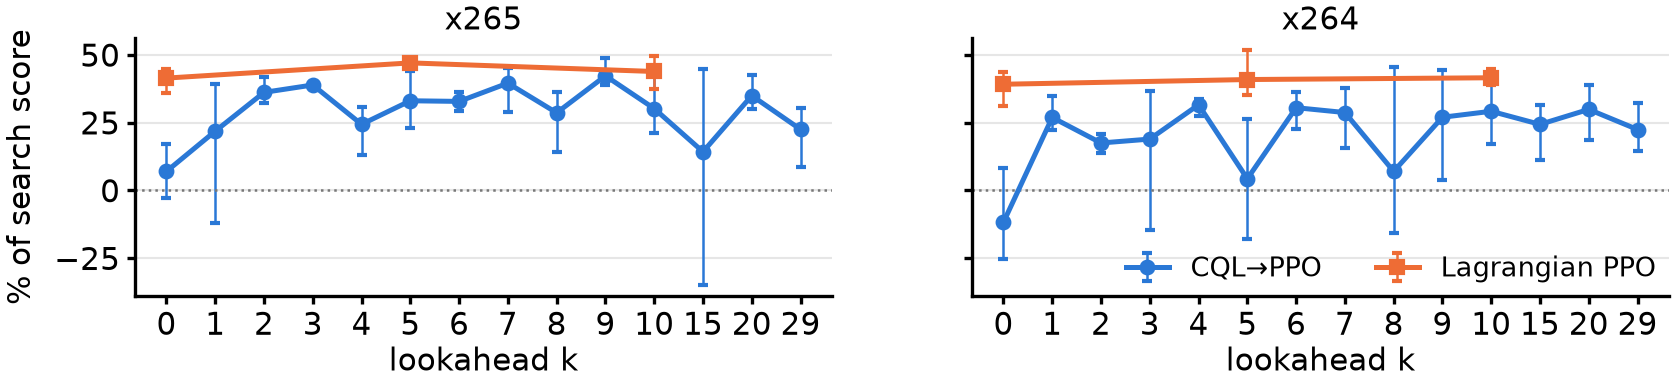
\includegraphics[width=0.78\linewidth]{fig_lookahead.png}
\caption{Share of the search's score captured against lookahead $k$ (mean of 3 seeds; bars: seed range).}\label{fig:la}
\end{figure}

\subsection{Over-budget behaviour of CQL$\to$PPO}
x265, share of GOPs over / mean \% over / p95 \% over: $k=0$ QP 30: 33\% / 2.33 / 14.2; QP 38: 22\% / 0.91 / 6.3;
$k=5$: 21\%/0.89/5.2 and 20\%/0.78/4.8; the lowest is $k=7$ at QP 38 (3.5\%, p95 0).

\subsection{Feature ablations ($k=5$, CQL$\to$PPO)}
\begin{center}\small
\begin{tabular}{lrr|lrr}
\toprule
Dropped & x265 & x264 & Dropped & x265 & x264 \\\midrule
none (all) & 3.48 & 0.43 & fp, pixel, scene & $-3.62$ & $-5.61$ \\
first pass (fp) & $-0.97$ & $-1.07$ & history, fp, pixel & $-4.38$ & $-8.66$ \\
history & 1.92 & 1.57 & history, fp, scene & $-1.07$ & $-2.80$ \\
pixel & 1.81 & 3.15 & history, pixel, scene & 2.63 & $-0.70$ \\
scene & 3.40 & 3.23 & all four & $-4.41$ & $-2.94$ \\
all + scene budget prior & 3.22 & 3.02 & & & \\
\bottomrule
\end{tabular}
\end{center}
First-pass cost is the feature that matters (+4.45 [+3.42, +5.80] on x265, clip-level). On x264, dropping pixel or
scene features \emph{raises} the score, because the full-feature x264 $k=5$ run is one of the collapsed points.

\subsection{Scene-aware and dynamic lookahead}
\begin{center}\small
\begin{tabular}{lrrr|rrr}
\toprule
& \multicolumn{3}{c|}{x265} & \multicolumn{3}{c}{x264} \\
Policy & score & frames seen & $>$1\% over & score & frames seen & $>$1\% over \\\midrule
CQL$\to$PPO $k=0$ & 0.74 & 0 & 22\% & $-1.17$ & 0 & 25\% \\
CQL$\to$PPO cut-triggered (cap 5) & 3.32 & 0.2 & 10\% & 1.67 & 0.2 & 16\% \\
CQL$\to$PPO fixed $k=5$ & 3.48 & 4.5 & 15\% & 0.43 & 4.5 & 24\% \\
CQL$\to$PPO scene-truncated 5 / 10 & 3.91 / 3.00 & & 14 / 16\% & 3.07 / 3.56 & & 14 / 16\% \\
CQL$\to$PPO scene-extended 5 / 10 & 3.19 / 4.06 & & 13 / 6\% & 2.57 / 2.84 & & 16 / 15\% \\
any-$k$ policy at $k=$ 0 / 2 / 3 / 5 / 7 & \multicolumn{3}{l|}{1.58 / 3.62 / 4.02 / 4.50 / 3.74} & \multicolumn{3}{l}{0.40 / 3.14 / 3.79 / 3.80 / 4.00} \\
any-$k$ at $k=$ 10 / 15 / 20 / 29 & \multicolumn{3}{l|}{2.81 / 2.33 / 1.87 / 1.51} & \multicolumn{3}{l}{3.36 / 0.27 / 1.82 / 3.20} \\
any-$k$ scene-truncated 5 & 4.56 & & 3\% & 3.92 & & 4\% \\
\bottomrule
\end{tabular}
\end{center}
Cut-triggered vs $k=0$: +2.58 [+1.80, +3.23] (x265), +2.84 [+1.98, +3.97] (x264); natural GOPs only +2.39, +2.21;
x264 seeds +5.08, $-0.92$, +4.36. \emph{Caveat:} ``frames seen'' excludes the scene detector's own scan; the trigger
needs to know a cut is within 5 frames, so the real delay saving is not yet measured. Scene-truncated vs fixed
$k=5$: +0.43 [+0.15, +0.80] (x265), +2.64 [+2.10, +3.33] (x264). The lookahead rule's own cut-triggered mode does not
help ($-5.76$ x265). The any-$k$ policy is the strongest single network (4.50 at $k=5$, 3\% over, x265).

\subsection{Extensions (D23) and model-based pre-training (D26)}
\begin{center}\small
\begin{tabular}{lrr|lrr}
\toprule
Method ($k=5$ unless noted) & x265 & x264 & Method & x265 & x264 \\\midrule
CQL$\to$PPO (reference) & 3.48 & 0.43 & ensemble of 3 seeds & 4.52 & 3.44 \\
CQL$\to$A2C & 1.79 & 1.48 & gate $\lambda=1$ / 3 & 3.17 / 3.38 & 1.09 / 0.41 \\
CQL$\to$DQN & $-1.72$ & $-1.72$ & Lagrangian / PID fine-tune & 4.10 / 4.03 & 4.13 / 3.17 \\
+fb features & 2.72 & 2.50 & \code{mb} $k=0$ / 5 & $-0.73$ / 0.61 & $-0.54$ / $-0.42$ \\
+sum features, $k=5$ / 29 & 3.40 / 3.68 & 3.44 / 3.93 & \code{mb\_ppo} $k=0$ / 5 & 0.69 / 0.96 & 0.09 / 1.00 \\
\bottomrule
\end{tabular}
\end{center}
Model-based pre-training history: v1 diverged (in-model score 9.7 within 25k steps, then $-\infty$ saving and NaN
logits; the policy exploited the model); v2 anchors the model to the GOP's real STATIC encode, adds noise (GOP bias sd
0.10, frame sd 0.05 in log2 bits) and bounds PSNR delta and score. On val the model scores a CQL$\to$PPO policy at 11.3
vs 12.9 real (corr 0.60, MAE 13.7 points per GOP). Outcome: stable, cuts CQL's over-budget rate from 26--29\% to
7--16\% but the saving drops to 1--1.7\%; the model learns ``spend less''. Lesson: accuracy relative to the
decision's effect, not simulator cost, is the binding constraint.

MPC history: v1 was over budget on 60--80\% of GOPs (CEM pushes predicted PSNR to the predicted budget and picks plans
the model underestimates, though the model is unbiased: actual/predicted median 1.03, p10--p90 0.88--1.19); v2 plans
against a margin (every x265 run chose 0.80, the lowest offered), v3 widened the grid to 0.60--1.0. MPC stays below
constant QP.

\subsection{Where the $k=5$ policy wins (x265, vs the $k=5$ lookahead rule, saving clipped $\pm$50)}
Strong hard cuts +9.64 (40 GOPs), moderate cuts +7.95 (26), high-motion no-cut +5.38 (174), fades +3.99 (65),
low-motion no-cut +3.71 (174). Largest losses: two UGC animation GOPs ($-9.9$, $-7.0$) and two Sintel fades
($-4.5$, $-4.2$). Learned vs hand lookahead rule at $k=5$: +5.99 [+4.77, +7.48] (clip-level).

\subsection{Cross-codec comparison}
On a common yardstick (x264's bits/PSNR scored on x265's constant-QP curve), x264's constant QP scores $-29.3$ (saving
$-9.6$\%): the codec gap. Points whose PSNR falls outside x265's QP 18--50 range are left out (D22; log-bits
extrapolation had given $-1379$ and $-3\times10^{11}$); x264 ABR+AQ loses 127 of 958 points that way.
\emph{Known issue:} the RL rows of \code{codecs\_report.md} predate the 31 Oct \code{analysis.py} fix (x265 $k=5$ shows
3.20 instead of 3.48); the lookahead and methods reports are authoritative.

%=====================================================================
\section{Multi-GOP streams (\#2, D25) and the fair head-to-head (D29)}
\textbf{Setting.} 8 IDR GOPs (same-clip time-ordered or mixed clips) under one budget $s\times$ bits at constant QP
$q_0$ (train $q_0\in$ 24--44, $s\sim U(0.8,1.25)$; eval $q_0\in\{30,38\}$, $s\in\{0.85,1.0,1.18\}$); 152 test streams,
912 cases. Each step picks a GOP's constant QP as an offset $-6..+6$ on a causal model QP (5.5 QP per doubling,
online calibration). Outcomes from the real constant-QP curves (exact, no encodes). PSNR pooled over MSE (a dB mean
gave the hindsight plan a spurious +36\%). Score 0 = best constant QP in hindsight.

\textbf{D29.} The encoders code each stream as one 240-frame encode (IDR every 30, closed GOPs) at the budget as
average bitrate (frame rate set so kbps/fps equals budget/240 exactly). Checks: the stream encode at constant QP
reproduces the per-GOP curve bits exactly (x265) / within 0.3\% (x264). Both encoders clamp rc-lookahead to keyint
(30), so the ``90-frame'' configs equal the 30-frame ones. CIs: 138 clusters.
\begin{center}\small
\begin{tabular}{lrrr|rrr}
\toprule
& \multicolumn{3}{c|}{x265} & \multicolumn{3}{c}{x264} \\
Method & score & saving & $>$1\% over & score & saving & $>$1\% over \\\midrule
our rule (model QP), $L=0$ / 2 & $-20.68$ / $-10.37$ & & 27\% & $-44.86$ / $-14.08$ & & 33--34\% \\
BC, $L=0$ / 2 & $-16.99$ / $-19.56$ & & 10 / 7\% & $-16.06$ / $-19.63$ & & 9 / 7\% \\
PPO, $L=0$ / 2 & 0.96 / 3.04 & 1.05 / 3.13 & 2 / 1\% & $-0.77$ / 1.87 & & 2 / 1\% \\
BC$\to$PPO, $L=0$ & 1.65 & 1.70 & 1\% & 0.11 & 0.47 & 2\% \\
BC$\to$PPO, $L=2$ & 3.23 & 3.28 & 1\% & 1.86 & 2.06 & 1\% \\
Encoder ABR & $-37.53$ & $-13.35$ & 64\% & $-29.61$ & $-10.24$ & 70\% \\
Encoder ABR + cutree/mb-tree & $-21.65$ & $-0.73$ & 34\% & $-13.42$ & $-0.61$ & 45\% \\
Encoder ABR + AQ & $-23.52$ & $-2.51$ & 34\% & $-18.81$ & $-8.37$ & 41\% \\
Encoder plain two-pass & $-2.30$ & $-0.38$ & 30\% & 0.57 & 1.94 & 22\% \\
Encoder two-pass + default AQ & 3.83 & 7.03 & 45\% & 3.18 & 4.49 & 22\% \\
Hindsight per-GOP plan & 12.54 & 12.54 & 0\% & 12.45 & 12.46 & 0\% \\
\bottomrule
\end{tabular}
\end{center}
Paired (x265): BC$\to$PPO $L=0$ vs ABR+cutree +23.30 [+18.68, +28.48] score, +2.43 [+1.26, +3.74] saving; $L=2$
+24.88 / +4.01; vs AQ ABR +25.16 / +4.22; BC$\to$PPO $L=2$ vs plain two-pass +5.53 [+4.46, +6.54]; hindsight plan vs
two-pass +14.84. x264: vs ABR +29.71; vs ABR+mb-tree +13.5, saving +1.1 (n.s.); vs two-pass +1.3. Remaining bias
favours the encoder (it picks a QP per frame, RL one per GOP). The hindsight plan often runs below budget because the
score does not reward using it (an early sign of the issue in Section~\ref{sec:under}).

%=====================================================================
\section{Wide-budget study (D28, QP 26--42)}
Budgets at QP 26, 30, 34, 38, 42 (a 4$\times$ bitrate range); continuous budget input
$(b-\min)/(\max-\min)$; extra STATIC encodes and search only at 26/34/42 (exact reuse of 30/38); 69 RL runs per encoder.
\begin{center}\small
\begin{tabular}{lrrrrrr|rrrrrr}
\toprule
& \multicolumn{6}{c|}{x265} & \multicolumn{6}{c}{x264}\\
Method & 26 & 30 & 34 & 38 & 42 & all & 26 & 30 & 34 & 38 & 42 & all \\\midrule
STATIC & $-5.3$ & $-10.5$ & $-13.0$ & $-16.9$ & $-22.0$ & $-13.5$ & $-8.8$ & $-11.9$ & $-14.9$ & $-20.0$ & $-23.9$ & $-15.9$ \\
BC $k=0$ & 2.27 & 1.67 & 1.33 & 0.31 & $-2.52$ & 0.61 & 1.74 & 0.89 & 1.66 & $-0.76$ & $-2.27$ & 0.25 \\
CQL$\to$PPO $k=0$ & 4.19 & 4.31 & 3.37 & 2.53 & 0.00 & 2.88 & 2.48 & 3.02 & 2.56 & 1.59 & $-0.54$ & 1.82 \\
CQL$\to$PPO $k=5$ & 4.84 & 4.93 & 4.19 & 3.59 & 2.42 & 3.99 & 2.12 & 3.21 & 3.58 & 3.10 & 1.93 & 2.79 \\
Lagrangian $k=0$ & 4.59 & 4.60 & 4.25 & 4.02 & 2.87 & 4.07 & 4.37 & 5.11 & 4.58 & 3.85 & 3.60 & 4.30 \\
Lagrangian $k=10$ & 5.30 & 5.05 & 4.36 & 4.05 & 3.04 & 4.36 & 4.36 & 5.53 & 4.39 & 3.46 & 3.46 & 4.24 \\
PID $k=5$ & 5.05 & 5.13 & 4.42 & 4.39 & 3.56 & 4.51 & 4.85 & 5.28 & 4.49 & 3.74 & 2.92 & 4.26 \\
Hindsight search & 10.22 & 10.96 & 10.38 & 10.10 & 9.41 & 10.22 & 9.21 & 10.04 & 10.03 & 9.86 & 9.88 & 9.80 \\
\bottomrule
\end{tabular}
\end{center}
Findings: the search gains $\approx$10 at every budget; constrained RL is best at every budget; its lead over BC grows
as budgets tighten (Lagrangian $-$ BC at $k=0$, x265: +2.3 at QP 26 to +5.4 at QP 42); lookahead is worth more at tight
budgets; five-budget training mainly fixes CQL$\to$PPO's overshoot ($k=0$ at QP 30/38: x265 0.74 $\to$ 3.42, x264
$-1.17\to$ 2.31). Budgets stop at 26/42 because plan QPs reach 17 and 48, near the curve range.

%=====================================================================
\section{Validity review and re-analysis (D30)}\label{sec:reanalysis}
\subsection{Holes we found in our own setup}
(Partly from Aayush's code review, \code{/scratch1/aayushso/ee599/docs/msg-pavneet-2026-11-03.md}, and partly our own.)
\begin{enumerate}
\item Learners are given the base QP that exactly meets the budget (an oracle).
\item The budget is derived from the GOP's own cost, so it reveals that cost even at $k=0$.
\item Some scene flags used up to 4 later frames.
\item Early intervals treated cases as independent, though test GOPs come from 38 clips and 60 splices.
\item Splices are artificial cuts. Also confirmed: STATIC is a weak reference.
\end{enumerate}
\subsection{Clip-level re-analysis of every headline (original setting)}
\begin{center}\small
\begin{tabularx}{\linewidth}{Lrrl|rrl}
\toprule
& \multicolumn{3}{c|}{x265} & \multicolumn{3}{c}{x264} \\
Claim & A$-$B & clip CI & verdict & A$-$B & clip CI & verdict \\\midrule
Lagrangian beats BC, $k=0$ & +2.68 & [+1.89, +3.44] & holds & +3.68 & [+2.68, +4.62] & holds \\
Lagrangian beats BC, $k=5$ & +1.19 & [+0.49, +1.82] & holds & +1.42 & [+0.38, +2.22] & holds \\
Lagrangian beats BC+feedback, $k=0$ & +2.79 & [+2.00, +3.58] & holds & & & \\
Feedback helps BC, $k=0$ & $-0.10$ & [$-0.39$, +0.13] & n.s. & +0.39 & [+0.06, +0.71] & holds \\
Lagrangian beats CQL$\to$PPO, $k=5$ & +1.47 & [+1.02, +1.98] & holds & +3.64 & [+2.89, +4.55] & holds \\
CQL$\to$PPO beats BC, $k=5$ & $-0.28$ & [$-0.94$, +0.22] & n.s. & $-2.22$ & [$-3.32$, $-1.48$] & BC better \\
BC beats CQL, $k=5$ & +5.54 & [+3.59, +8.77] & holds & & & \\
Lookahead $k$ 0$\to$5 & +2.74 & [+1.79, +3.64] & holds & +1.60 & [+0.50, +2.78] & holds \\
Lookahead $k$ 3$\to$29 & $-1.73$ & [$-2.34$, $-1.19$] & holds & +0.35 & [$-0.67$, +1.06] & n.s. \\
Ensemble helps & +1.04 & [+0.69, +1.49] & holds & +3.01 & [+2.36, +3.97] & holds \\
First-pass features matter & +4.45 & [+3.42, +5.80] & holds & +1.50 & [+0.38, +2.90] & holds \\
Cut-triggered beats none & +2.58 & [+1.80, +3.23] & holds & +2.84 & [+1.98, +3.97] & holds \\
Gap: search $-$ Lagrangian $k=5$ & +5.58 & [+5.00, +6.32] & holds & +5.88 & [+5.14, +6.64] & holds \\
\bottomrule
\end{tabularx}
\end{center}
Seed spread reaches 4.5 points; clip-level CIs average seeds first, so they omit it. BC + feedback control
(\code{policies.Feedback}, gain and margin tuned on val; the feedback rule's gain was tuned on validation and chose 2)
is the non-RL answer to ``is RL needed for the budget?''.

\subsection{Causal environment}
\code{RC\_CAUSAL=1}: budget $= s\times$ constant-QP bits at $b$ with $s$ unknown (train $U(0.8,1.25)$, eval one of
0.85/1.0/1.18 per case by hash); base QP from a first-pass STATIC rate model fitted on train
(\code{causal\_prior.json}); per-frame cost features normalised by $B/30$; cut/flash/fade flags recomputed from
visible frames only; offline plans re-expressed as offsets on the model base QP (plans leaving $-3..3$ dropped). A
per-frame base QP was rejected ($\pm$2 for only 25\% at $k=0$). GOP-level rate model accepted: base QP within $\pm$2 of
$b$ for 75\% (x265 test) / 66\% (x264); mean error +0.27 / +0.32; 54\% / 46\% of logged plans kept; at $k=0$ the stored
flags differ from what the detector knows on 2.4\% of test frames. MPC, \code{mb} and gate are not ported.

%=====================================================================
\section{Causal rerun (five budgets, hidden budget scale)}
2,395 test cases (479 GOPs $\times$ 5 budgets); x265 39 RL runs + 24 learning-curve runs, x264 39 runs. Constant QP
at $b$ is no longer 0 because the budget is scaled ($-11.44$, 32\% over).
\begin{center}\small
\begin{tabular}{lrrr|rrr}
\toprule
& \multicolumn{3}{c|}{x265} & \multicolumn{3}{c}{x264} \\
Method & score & saving & $>$1\% over & score & saving & $>$1\% over \\\midrule
STATIC on causal base QP & $-19.37$ & 1.11 & 52\% & $-21.90$ & 1.01 & 54\% \\
Feedback rule $k=0$ & $-15.43$ & $-1.47$ & 59\% & $-20.52$ & $-1.55$ & 60\% \\
Lookahead rule $k=5$ & $-3.82$ & $-0.36$ & 20\% & $-7.09$ & $-0.80$ & 25\% \\
BC $k=0$ / 5 & $-5.01$ / $-4.39$ & 1.49 / 2.22 & 24\% & $-13.18$ & 1.54 & 32\% \\
CQL$\to$PPO $k=0$ / 5 & 1.03 / 1.42 & 3.00 / 3.50 & 6\% & $-3.40$ / $-3.29$ & 2.36 / 3.03 & 12--13\% \\
Lagrangian $k=0$ / 5 & 1.07 / 1.26 & 3.06 / 3.20 & 4--5\% & $-2.36$ & 2.55 & 8\% \\
PID $k=0$ / 5 & 1.24 / 1.02 & 3.39 / 3.98 & 5--9\% & & & \\
Hindsight search & 3.81 & 10.32 & 26\% & 3.68 & 9.93 & 26\% \\
Encoder two-pass + AQ & $-17.37$ & $-1.10$ & 57\% & $-12.79$ & $-4.93$ & 29\% \\
\bottomrule
\end{tabular}
\end{center}
Clip-level claims (x265 / x264): Lagrangian beats BC at $k=0$ +6.09 [+4.81, +7.84] / +10.82 [+8.06, +14.97]; at $k=5$
+5.65 / +7.54; holds on natural GOPs and every seed. Feedback helps BC +0.94 [+0.37, +1.78] / +4.36 [+2.15, +8.29].
On x265, Lagrangian beats BC + feedback by +5.14 ($k=0$) and +4.39 ($k=5$). Lookahead CQL$\to$PPO $k$ 0$\to$5: +0.40 (case-level only) / +0.11
(n.s.); Lagrangian $k$ 0$\to$5: +0.18 / +0.02; the gain sits on spliced GOPs. Learned vs hand lookahead rule +5.25. Gap
search $-$ Lagrangian $k=5$: +8.93 / +10.59. Lagrangian vs encoder ABR +30.6 / +38.0, vs two-pass + AQ +18.6 / +10.6;
vs the best constant QP in hindsight only +1.07 [$-1.35$, +2.75] (case-level only). Caveat: the causal budget
($s\times$ the GOP's own spend) is still not leak-free by the v1 standard.

%=====================================================================
\section{Learning curve (D32)}
CQL$\to$PPO, causal x265, five budgets, trained on 12.5 / 25 / 50 / 100\% of whole training clips (nested per seed), 3
seeds, 24 runs (\code{results/x265\_causal/learning\_curve\_report.txt}).
\begin{center}\small
\begin{tabular}{lrrrr|rrrr}
\toprule
& \multicolumn{4}{c|}{$k=0$} & \multicolumn{4}{c}{$k=5$} \\
Share of clips & train & test & saving & over\% & train & test & saving & over\% \\\midrule
12.5\% & 2.67 & $-1.33$ & 3.00 & 16.5 & 3.58 & $-0.15$ & 3.63 & 16.8 \\
25\% & 2.27 & 0.65 & 2.97 & 6.1 & 1.70 & $-1.02$ & 3.07 & 14.1 \\
50\% & 1.31 & $-0.10$ & 2.57 & 9.4 & 2.20 & 0.63 & 3.23 & 10.7 \\
100\% & 1.68 & 1.03 & 3.00 & 6.7 & 2.18 & 1.42 & 3.50 & 7.6 \\
\bottomrule
\end{tabular}
\end{center}
100\% minus 50\%: +1.13 [+0.68, +1.77] ($k=0$), +0.80 [+0.15, +1.39] ($k=5$). Saving is flat; the over-budget share
falls by more than half; the train--test gap falls from about 4 to under 1. Not monotonic, with seed spread up to 4.4
at small shares. Conclusion: more clips buy budget reliability, not compression.

%=====================================================================
\section{Dataset v1 (D31)}
\subsection{Dataset and port}
Aayush's dataset v1: 109 clips from 78 sources, 1,042 GOPs (625 train / 152 val / 265 test; 66/16/27 clips),
human-checked cuts, splices in train only, split by source group. Leak-free clip-level budgets: for each level
$q\in\{24,30,36,42\}$, the mean over the clip's GOPs of constant-QP bits. Frozen encoder settings: preset medium,
IPPP, AQ/mb-tree/psy off. Our pipeline reads his clips, GOP files, manifest and budgets read-only and writes to
\code{rcwork\_v1/<codec>} and \code{results/v1/<codec>}. Action: residual $-3..+3$ on his causal online controller,
ported to \code{rclib/controller.py} (margin 0.97, dI 3, i\_cap 1.0, w0 2, dmax 3, fcap 4, pmin 1, wfp 2), which
solves before each frame for the P-frame QP that spends margin $\times$ the remaining budget under a rate model fitted
on train with online updates. Residual was chosen because a $\pm$3 action on a fixed base cannot reach the budget at
$k=0$ (base-QP error 3.6--4 QP); a $\pm$8 action range was rejected. Internal success rule (kept internal): at least
1 point, clip-level CI excludes 0, all seeds agree.

\subsection{Debug and the search fix}
x265 debug 13754428 verified the port (budget / own spend 1.04; controller $-3.12$ at $k=0$ and $-0.30$ at $k=5$ with no
overshoot; prefix property holds; 0.23 s per encode at preset medium), but only 4--5\% of search plans fitted $\pm$3
around the controller and the search from STATIC scored badly. Fix: the search starts from the controller's $k=29$
plan and clips residual targets. Re-tests: x264 13754429 (4:35; controller $-4.20$/$-1.05$ vs Aayush's
$-3.94$/$-0.94$; plans inside $\pm$3: 30\%/40\%); x265 13757091 (6:25; 46\%/50\%; frames inside 90--91\%).

\subsection{Stage 1 results (old score; test, difference vs the controller, source-group bootstrap)}
\begin{center}\small
\begin{tabular}{lrrr|rrr}
\toprule
& \multicolumn{3}{c|}{x265} & \multicolumn{3}{c}{x264} \\
Method, $k$ & test & diff & 95\% CI & test & diff & 95\% CI \\\midrule
Controller, 0 / 5 & $-3.86$ / $-0.38$ & & & $-3.67$ / $-1.13$ & & \\
BC, 0 & $-24.72$ & $-20.86$ & [$-26.6$, $-10.2$] & $-13.76$ & $-10.09$ & [$-15.0$, $-4.3$] \\
BC, 5 & 1.59 & +1.97 & [+1.10, +2.88] & 1.84 & +2.97 & [+2.09, +3.80] \\
CQL$\to$PPO, 0 & $-0.20$ & +3.66 & [+2.45, +5.81] & $-0.95$ & +2.72 & [+1.68, +3.56] \\
CQL$\to$PPO, 5 & 1.65 & +2.02 & [+0.77, +3.17] & 2.37 & +3.50 & [+2.33, +4.60] \\
Lagrangian, 0 & $-0.74$ & +3.12 & [+1.93, +4.90] & $-1.01$ & +2.66 & [+1.56, +3.82] \\
Lagrangian, 5 & 2.40 & +2.78 & [+1.60, +3.65] & 2.11 & +3.24 & [+1.98, +4.34] \\
PID, 0 & $-1.31$ & +2.55 & [+1.41, +4.33] & $-2.13$ & +1.54 & [+0.11, +2.82] \\
PID, 5 & 0.54 & +0.92 & [$-0.45$, +2.24] & 1.30 & +2.43 & [+1.11, +3.68] \\
\bottomrule
\end{tabular}
\end{center}
CQL$\to$PPO and Lagrangian meet the internal rule at both $k$ on both encoders; BC only at $k=5$; PID $k=5$ fails on
x265. These results use the old score and are superseded by Section~\ref{sec:under}. Stage 2 (Lagrangian sweep $k=0,1,2,5,10,29$ with 5 seeds plus the
controller at $k=1,2,10,29$; 28 new runs per encoder) and Stage 3 (cut-triggered lookahead, ensembles) were prepared
but not submitted.

%=====================================================================
\section{Unused budget: the problem found today and D33}\label{sec:under}
\subsection{What we found}
Aayush reported that the score does not penalise unused budget: spending less at lower PSNR is free if the
efficiency is good, and his residual RL raised QP on 87\% of frames and used 66\% of the budget. Our score (saving at
equal PSNR $-$ 2 $\times$ \% over) has the same property. Measured on our test evaluations (3 seeds pooled),
against STATIC at the same budget level:
\begin{center}\small
\begin{tabular}{llrrrr}
\toprule
Setting & Method & spend/budget & $\Delta$PSNR vs STATIC & GOPs below STATIC & saving \\\midrule
Causal, x265 & BC $k=0$ & 0.912 & $-0.54$ dB & 69\% & 1.49 \\
& CQL$\to$PPO $k=0$ / 5 & 0.808 / 0.801 & $-1.01$ / $-1.00$ & 82 / 81\% & 3.00 / 3.50 \\
& Lagrangian $k=0$ / 5 & 0.782 / 0.784 & $-1.15$ / $-1.13$ & 85 / 85\% & 3.06 / 3.20 \\
& PID $k=0$ & 0.782 & $-1.14$ & 84\% & 3.39 \\
Causal, x264 & BC $k=0$ & 0.953 & $-0.53$ & 64\% & 1.54 \\
& CQL$\to$PPO $k=0$ / 5 & 0.844 / 0.846 & $-1.00$ / $-0.97$ & 78 / 78\% & 2.36 / 3.03 \\
& Lagrangian $k=0$ / 5 & 0.808 / 0.828 & $-1.20$ / $-1.07$ & 81 / 82\% & 2.55 / 2.73 \\
Original, x265 & BC $k=0$ & 0.922 & $-0.45$ & 81\% & 3.68 \\
& CQL$\to$PPO $k=0$ / 5 & 0.949 / 0.928 & $-0.30$ / $-0.32$ & 64 / 65\% & 3.97 / 5.11 \\
& Lagrangian $k=5$ & 0.871 & $-0.58$ & 84\% & 5.22 \\
Original, x264 & BC $k=0$ & 0.912 & $-0.59$ & 76\% & 3.12 \\
& CQL$\to$PPO $k=0$ / 5 & 0.963 / 0.959 & $-0.34$ / $-0.27$ & 76 / 61\% & 2.94 / 4.45 \\
& Lagrangian $k=5$ & 0.911 & $-0.48$ & 78\% & 4.79 \\
\bottomrule
\end{tabular}
\end{center}
The savings are real at matched quality, but at a lower operating point than the budget allows; the constrained
learners, best by score, under-spend most. The asymmetric penalty (2 per \% over, 0 per \% under) teaches a safety
margin. v1 Stage 1 has the same reward form (not measured).

\subsection{D33: under-budget penalty}
Score $-=$ \code{RC\_UNDER\_PENALTY} $\times\max(0,$ \% unused $-$ \code{RC\_UNDER\_TOL}$)$, set to 1 point per \% beyond
3\%; default 0 so earlier runs reproduce. It enters the search, the offline rewards (through the search logs), the
relative reward, and the Lagrangian objective (overshoot remains the constraint). New: \code{metrics.undershoot},
\code{metrics.under\_cost}, \code{under\_pct} in env results, spend/budget and PSNR-vs-controller columns in
\code{v1\_report.py}, \code{experiments/v1\_rescore.py} (copies v1 infos, scenes and controller plans and re-scores the
controller plan without re-encoding, since the search starts from that score), \code{tools/v1u\_debug.sbatch},
\code{tools/submit\_v1u.sh}. Old Stage 1 untouched.

\textbf{Debug (quick subset, pipeline check only):} x265 13992008 (5:58) and x264 13992454 (2:57; first attempt
13992009 failed because it pointed at \code{test2\_x264} instead of \code{test\_x264}). Controller score under the
penalty $-4.07\to-9.55$ (x265 quick). Spend/budget: controller 89.8\% / 94.5\%, quick Lagrangian 99.8\% / 103.5\% with
+0.29 / +0.23 dB vs the controller; the quick Lagrangian scores ($-13.73$/$-21.32$, 33--46\% over) are meaningless at
1,792 training steps.

\textbf{Full rerun submitted} (both encoders): rescore, search train/val/test (16/4/6 shards), 26 RL runs (13 at a
time), report. x265: 13993253--61; x264: 13993262--70. At writing, 9 x265 search shards were running and the rest
pending. Reports will go to \code{results/v1u/<codec>}.

\subsection{The teammate's rerun and how it differs}
Aayush's package (\code{/scratch1/aayushso/ee599/docs/review-pavneet-2026-11-10/}) reruns everything in a copy of our
code (branch \code{v1-data}, arms \code{orig/dec/lf/res/lfq}) with a quality-at-budget metric:
$\text{score} = \text{PSNR} - \text{PSNR}_{\text{CQP}}(B) - 0.17\,\text{dB}\times\%\text{over}$, where
$\text{PSNR}_{\text{CQP}}(B)$ is the constant-QP curve's PSNR at exactly the budget (0.17 dB $\approx$ the old 2 points
per \% converted at about 6 dB per doubling of bits). Under-spending is penalised automatically.
\begin{center}\small
\begin{tabularx}{\linewidth}{lLLL}
\toprule
& Ours (v1, and D33) & His \code{res} & His \code{lfq} (leak-free + quality metric) \\\midrule
Action & residual $-3..+3$ on our controller port & residual $-3..+3$ on his (retuned) controller & offset $-10..+10$ (21 actions) on causal base QP estimate + STATIC ramp \\
State & shared layout; slot 2 = controller QP, slot 15 unused & slot 15 = controller QP & slot 15 = causal base QP \\
Score & saving $-$ 2$\times$\%over ($-$ under penalty in D33) & dB at budget $-$ 0.17$\times$\%over & same \\
Lagrangian $\lambda$ & 4 points per \% & 0.34 dB per \% & 0.34 dB per \% \\
Reward baseline & none (v1) & controller's own result on that GOP, level, $k$ & search start plan (constant offset) \\
Reward scale & /10 & 1 & 1 \\
Controller & margin 0.97, dI 3, i\_cap 1.0, no ramp & retuned: margin 1.0, dI 9, ramp on & -- \\
Search & $\pm$3 around controller plan & -- & $\pm$5 around hindsight base, re-expressed on causal base, out-of-range plans dropped (3--4\%) \\
Data & v1 incl.\ flat GOPs & 13 flat GOPs excluded & same \\
Runs & $k=0,5$ $\times$ 3 seeds, 26 per encoder & $k$ 0/2/5/10/29 $\times$ 3 & 45 per encoder \\
\bottomrule
\end{tabularx}
\end{center}
His early numbers (x264): the search's best plan +0.17 dB at 99.6\% of the budget (the old leak-free search left 12\%
unused); its start plan $-0.25$ dB; the retuned controller $-0.22$ dB on test at 99.4\% of the budget (old setting
$-1.13$ dB on val); mean overshoot 0.91\% with 54\% of episodes slightly over. The headroom in dB is about 0.4 dB.
His review questions: (1) other places assuming rewards in points/10; (2) whether PPO entropy 0.01, CQL $\alpha$ 1.0,
distillation temperature 0.3 and value-from-Q need retuning for dB-scale rewards; (3) whether dropping out-of-range
plans biases CQL; (4) slot 15 reuse; (5) remaining hard-coded 7- or 11-action assumptions. He offers parallel tasks:
the review, dB tables and figures, or MPC on the leak-free setup ($\approx$30 CPU-h).

\textbf{Recommendation recorded:} adopt his metric and settings, cancel or hold the D33 rerun (it shares the account's
fairshare and yields non-comparable numbers), and take on the patch review. Pending the user's decision.

%=====================================================================
\section{Reports and documents produced}
\begin{itemize}
\item \textbf{Result reports} (\code{results/<codec>/}): infos, scenes, search, baselines, lookahead, expand2, methods,
features, scene, overshoot, breakdown, constraint, clip, own\_rc\_stream, reanalysis, codecs; \code{\_wide} versions
plus budgets; \code{\_causal} breakdown, reanalysis, causal\_prep, learning curve; \code{v1/<codec>/v1\_stage1\_report.md}.
\item \textbf{Paper} \code{paper/paper.tex}$\to$\code{paper.pdf} (IEEEtran; 9 pages on 31 Oct, 10 on 2 Nov, 11 on 4 Nov
with related work on Mao et al.\ and MuZero rate control, scene-cut tables, cut-triggered lookahead and threats to
validity). Figures from \code{paper/make\_figs.py}, built from the reports only.
\item \textbf{3-page results report} \code{paper/report3/report.pdf} (numbers from \code{extract.py}$\to$\code{data\_*.json}).
\item \textbf{Milestone reports (Word):} \code{paper/milestone\_x265.docx}; \code{paper/milestone2/milestone\_report.docx}
(4 Nov); \code{paper/milestone3/milestone\_report.docx} (5 Nov, \code{tools/milestone3\_docx.py}): introduction,
related work (classical RC, learned RC; Mao et al.\ and MuZero for discussion only), methodology, setup, Table 1 (all
methods), Figure 1 (share of search score with seed ranges), Table 2 (dynamic lookahead), Table 3 (head-to-head),
discussion (what did not work; holes 1--5), plan (``Remaining work'' and ``Further analyses''), Appendix A
(baselines), Appendix B (work split, to be confirmed by the team). Edits made on request: ``To our knowledge''
removed; no mention of v1, Aayush's controller results, a new dataset, or success criteria; future work reads as
future work; dynamic lookahead added to show the proposal feedback was acted on. Page count checked by a XeLaTeX
proxy (4 pages), not in Word.
\item \textbf{Feedback received:} \code{Submission\_Feedback.docx} (TA), \code{milestone\_feedback\_from\_claude.docx},
\code{feedback2.docx}, \code{feedback3.docx} (its request to describe a second dataset was not applied, by the user's
later instruction).
\item \textbf{Team work split (draft, Appendix B):} Aayush -- dataset, scene labels, leak-free budgets, causal base QP;
controller, baselines, safety layer, MPC. Ahhana -- encoder wrapper, Gym env, frozen settings; A2C, DQN. Atharva --
hindsight search, wider budgets, evaluation; BC, CQL, IQL. Pavneet -- CARC pipeline, encoder head-to-head, clip-level
re-analysis; BC$\to$PPO, CQL$\to$PPO, lookahead sweep, causal rerun. Sara -- RL training setup, lookahead features,
budget handling; PPO, Lagrangian, PID-Lagrangian.
\end{itemize}

%=====================================================================
\section{Bugs, failures and fixes}
\begin{longtable}{p{4.2cm}p{12.2cm}}
\toprule
Problem & Fix / outcome \\\midrule
x264 ignores qpfile under \code{--qp} & carrier mode \code{--crf} with AQ and mb-tree off (L3). \\
ffmpeg psnr pairs frames by timestamp & \code{setpts} on both inputs. \\
x265 job failures (libstdc++) & \code{module load gcc/13.3.0} in \code{job\_env.sh}. \\
oneweek QOS submit cap & large arrays to \code{main} only. \\
Sintel URL 404 & 1080p mkv streamed through the downscaler. \\
SIGBUS (exit 135) on d11-41, d11-22 and all \code{xeon-4116} nodes & EPYC constraint on all jobs. \\
x264 RL run hung 6.9 h (likely SubprocVecEnv start-up deadlock) & cancelled, retries with a 2 h cap. \\
x264 own-RC shards failed; two-pass fails at very low targets & per-GOP failures allowed and counted. \\
Reports of both encoders overwrote each other & per-encoder folders \code{results/x265}, \code{results/x264}. \\
Codecs common-yardstick extrapolation ($-1379$, $-3\times10^{11}$) & out-of-range points excluded (D22). \\
DQN learned little (1k gradient steps) & one gradient step per transition (D21). \\
MPC over budget 60--80\% & margin chosen on val (D20), grid widened (D24). \\
Model-based PPO exploited the model (NaN) & anchoring, noise, bounded deltas (D26 v2). \\
\code{analysis.py} merged fb/sum runs into CQL$\to$PPO & configuration key includes \code{extra}; reports regenerated
(x265 $k=5$ 3.20$\to$3.48, $k=29$ 3.02$\to$2.37); \code{codecs\_report.md} RL rows still stale. \\
Multi-GOP dB-mean PSNR (+36\% artefact) & MSE pooling. \\
v1 search fitted 4--5\% of plans & search anchored at the controller's plan. \\
Own overclaim on dynamic lookahead (``reduces delay'') & corrected: detector scan not counted; one x264 seed below $k=0$. \\
Under-spending reward & D33 penalty; teammate's dB metric recommended. \\
D33 x264 debug pointed at wrong source dir & \code{RC\_SRC} override, resubmitted. \\
\bottomrule
\end{longtable}

%=====================================================================
\section{Decision log (D1--D33)}
\begin{longtable}{p{1cm}p{15.4cm}}
\toprule
ID & Decision \\\midrule
D1 & Paths on \code{/scratch1}; backups to \code{/home1/pbanga/ee599\_backup}. \\
D2 & Conda env by prefix, Python 3.12, latest packages. \\
D3 & Encoder PATH inside job scripts, never \code{.bashrc}. \\
D4 & Encode-heavy stages as job arrays; PPO one job per $(k,\text{seed})$; per-job recipe unchanged (RC\_ENVS 14, n\_steps 64). \\
D5 & Centre-crop to 16:9, scale to 320$\times$180, all frames kept. \\
D6 & Data sources (Xiph, films, UGC); runbook's unnamed pilot clips replaced. \\
D7 & STATIC $-6/-3/+3$ split at frame 10; refit studied. \\
D8 & Action $-3..+3$ on base QP + STATIC. \\
D9 & Bits from the Annex-B bitstream for both encoders. \\
D10 & 6:1:1 YUV PSNR, mean over frames. \\
D11 & Preset fast, first pass ultrafast, single-threaded. \\
D12 & GOP windows and spliced GOPs (120/40/60). \\
D13 & Splits by source; films whole. \\
D14 & Budget = own constant-QP bits at 30/38; score = saving $-$ 2 $\times$ \% over. \\
D15 & Offline cap 24 best + 24 random plans per (GOP, budget). \\
D16 & Runbook's 13 historical steps restructured into phases. \\
D17 & Strict lookahead. \\
D18 & Lookahead rule and scene rule as non-learned counterparts. \\
D19 & MPC with learned model + CEM. \\
D20 & MPC plans against a margin chosen on val. \\
D21 & DQN update rate. \\
D22 & Common-yardstick scores skip extrapolation. \\
D23 & Extensions: breakdowns, fb/sum features, CQL$\to$A2C/DQN, ensemble, gate, Lagrangian/PID fine-tunes. \\
D24 & MPC margin grid 0.60--1.0. \\
D25 & Multi-GOP rate control on exact curves. \\
D26 & Model-based pre-training (\code{mb}, \code{mb\_ppo}). \\
D27 & Constrained RL vs imitation analysis. \\
D28 & Wide-budget study (QP 26--42). \\
D29 & Fair head-to-head with the encoders' own RC on streams. \\
D30 & Validity fixes: clip-level re-analysis, BC + feedback, causal environment. \\
D31 & Dataset v1 in stages, residual RL on the causal controller, internal success rule. \\
D32 & Learning curve before any dataset expansion. \\
D33 & Under-budget penalty (1 point per \% beyond 3\%), first used on the v1 Stage 1 rerun. \\
\bottomrule
\end{longtable}

%=====================================================================
\section{Compute}
From \code{sacct} (29 Oct -- 10 Nov): about 1,280 job allocations (array tasks counted individually), about 9,800
CPU-hours outside the interactive session; 1,201 completed, 39 failed, 13 timed out, 1 out of memory, 10 cancelled.
Finished RL runs (evaluation files): original x265 277, x264 274; wide 81 + 81; causal x265 63 (incl.\ 24 learning
curve), x264 39; v1 26 + 26. Total about 870.

%=====================================================================
\section{Open items and pending decisions}
\begin{enumerate}
\item Decide on the D33 rerun (cancel or keep) and whether to adopt Aayush's dB metric and controller settings.
\item Reply to Aayush: which parallel task we take (patch review, dB tables/figures, or MPC on leak-free data).
\item Hold until the reward is settled: v1 Stage 2 and 3, learning curve on v1, BC + feedback on v1, Lagrangian on
streams, encoder-tools test (AQ/mb-tree on, \code{--zones}), VMAF, CRF baseline, RecurrentPPO, dense reward shaping,
delay cost of dynamic lookahead.
\item Git: nothing committed since 20c3862; no push without approval.
\item Deleting \code{/scratch1/pbanga/rcwork\_wide\_test} awaits approval.
\item Team to confirm the milestone 3 work split (Appendix B, Table A2).
\item Regenerate \code{codecs\_report.md} so its RL rows match the fixed analysis.
\end{enumerate}

\appendix
\section{Where things are}
\begin{tabularx}{\linewidth}{lL}
\toprule
Code & \code{rclib/} (config, codec, data, features, metrics, env, search, offrl, policies, mpc, mbenv, clipenv, controller,
runner), \code{experiments/} (infos, scenes, search, baselines, rl, analysis, reports, breakdown, codecs, constraint,
clip\_rl, own\_rc\_stream, reanalysis, bc\_feedback, causal\_prep, widen, budgets, reports\_wide, v1\_prep, v1\_report,
v1\_rescore), \code{tools/} (job\_env, step/rl\_batch sbatch, submit scripts, debug sbatch, docx builders, page check). \\
Run lists & \code{runs/} (core, methods, features, scenes, fix\_dqn\_mpc, mpc\_margin, extend, mb, mb\_ppo, wide, causal,
learning\_curve, v1\_stage1, v1\_stage2). \\
Docs & \code{docs/} JOURNAL, DECISIONS, LEARNINGS, JOBS, STUDY\_PLAN; \code{README.md}; \code{REPRODUCE\_HPC.md}. \\
Results & \code{results/\{x265,x264\}[\_wide|\_causal]}, \code{results/v1/}, \code{results/v1u/} (pending). \\
Work dirs & \code{/scratch1/pbanga/rcwork*}, \code{/scratch1/pbanga/rcwork\_v1/*}. \\
Teammate (read-only) & \code{/scratch1/aayushso/ee599/...}, \code{/scratch1/aayushso/rcwork\_v1/...}. \\
\bottomrule
\end{tabularx}
\end{document}
